\chapter{Theoretical foundation}
\label{ch:theory}

This chapter introduces the basic theoretical concepts that serve as a foundation for the problem definition and solution approach of this thesis. The problem we study is assisted lane keeping with shared control by a potentially distracted human driver and an agent. The agent acts as a lane-keeping assistant. The driver's attention and the exact position of the vehicle are unknown to the agent. The task involves sequential decision making, where every prior decision influences the following ones. Section \ref{sec:mdp} shows how sequential decision making tasks can be formulated using \Glspl{mdp}. However, since the agent only observes partial information, uncertainty about the driver's attentiveness and the car's road position is involved. Section \ref{sec:pomdp} introduces the \Gls{pomdp}, which is an extension of an MDP, accounting for partial observability of information. It is well suited to model the uncertainty involved in the problem. Solving POMDP is a difficult task. Section \ref{sec:challenges} discusses the key challenges involved in solving POMDP. Section \ref{sec:solvers} provides an overview of POMDP solvers.

\section{Sequential decision making}
\label{sec:mdp}

Lane-keeping of a car is a sequential decision-making task. Every steering action directly influences the choice of the best succeeding steering actions. \Glspl{mdp} are well suited and widely used to model sequential decision-making tasks. An \gls{mdp} is a discrete-time framework for a decision maker, the agent, to interact with an environment. Figure \ref{fig:mdp} illustrates the process. At every time step $t$, the environment is in a certain state $s_t$, fully observable by the agent. The agent interacts with the environment by performing an action $a_t$ that determines the next state $s_{t+1}$ of the environment. The underlying assumption, the Markov property, is that the next state of the environment only depends on its current state and the agent's action. The transition to a succeeding state does not need to be deterministic but can be probabilistic, accounting for randomness in the environment. After performing an action $a_t$, leading to state $s_{t+1}$, the agent receives a numerical reward $r_{t+1}$ (also called return). The agent's goal is to maximize the cumulative reward it receives over time. An action that leads to a high immediate return is not optimal if another action leads to a higher cumulative reward in the long run. Thus, the agent needs to find an optimal policy that decides the best action to take in every state. If the state transition probabilities are known to the agent, the optimal policy can be found using model-based techniques such as value or policy iteration. If the transition model is unknown, model-free reinforcement learning can be applied to learn an optimal policy.

\begin{figure}[htbp]
    \centering
    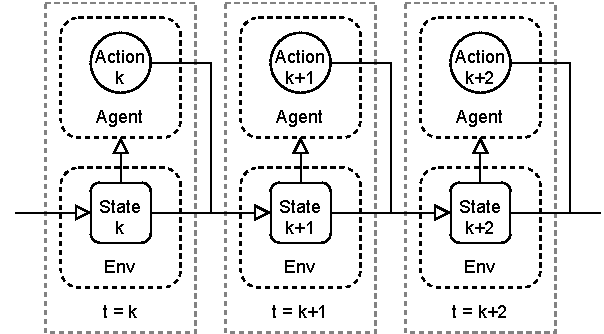
\includegraphics[width=0.75\textwidth]{figures/MDP.pdf}
    \caption{\acrfull{mdp}}
    \label{fig:mdp}
\end{figure}

\noindent
Assisting a human driver in the lane-keeping task is essentially a sequential decision-making task. However, the agent assisting the human driver does not know about the driver's internal psychological state. This state includes everything that influences the driver's behavior, such as the driver's goals, intentions, emotions, and perceptions, but is not visible from the outside world. We focus on the driver's attention to the driving task when referring to her hidden psychological state hereafter. A distracted driver may steer poorly and needs assistance. But how can the agent tell whether the driver is distracted? Reading the driver's mind is not feasible, and even if it were, it would be too invasive for this task. Instead, the agent needs to estimate the driver's internal state to act adequately. A \acrfull{pomdp} is a generalization of an MDP that allows planning under uncertainty. Even without observing the complete state of the agent's environment, a POMDP enables the agent to estimate the environment's true state using the partial information it observes. In the next section, we will give a formal definition of a POMDP.

\section{Partially observable Markov decision process (POMDP)}
\label{sec:pomdp}

A POMDP is a generalization of an MDP for planning under uncertainty. The environment's true state is unknown to the agent. It has to rely on observations with partial information about the environment's true state to choose its actions. We follow the description in \cite{pomdp-definition} and define a POMDP as a tuple $(S, A, T, R, O, Z)$, where:
\begin{itemize}
    \item $S$ is the set of all possible states $s \in S$ of the environment. A state describes the environment at a time point. It must not be an all-encompassing description but must include all relevant information to make decisions. The state is hidden from the agent. This is the main difference to an MDP.
    \item $A$ is the set of all possible actions $a \in A$ the agent can perform in the environment.
    \item $T : S \times A \times S \rightarrow [0,1]$ defines the conditional state transition probabilities. $T(s,a,s') = Pr(s' | s, a)$ constitutes the probability of transitioning to state $s'$ after performing action $a$ in state $s$.
    \item $R : S \times A \rightarrow \R$ is the reward function providing the agent with a reward of $R(s,a)$ after performing action $a$ in state $s$.
    \item $O$ is the set of all possible observations $o \in O$. Observations are the agent's source of information about the environment, enabling the agent to estimate the environment's state.
    \item $Z : S \times A \times O \rightarrow [0,1]$ defines the conditional observation probabilities. $Z(s', a, o) = Pr(o | s', a)$ represents the probability of receiving observation $o$ at state $s'$ after performing action $a$ in the previous state. 
\end{itemize}

\noindent
At any time, the environment is in a certain state $s$. Unlike in the case of an MDP, the agent cannot directly observe the environment's state. Instead, the agent receives an observation $o$ that provides partial information about the current state. The agent uses the observations it perceives over time to estimate the true state of the environment to choose adequate actions. At any time step $t$, it takes into account the complete history $h_t$ of actions and observations until $t$:

\begin{equation}
    h_t = \{a_0,o_1,...,o_{t-1},a_{t-1},o_t\}
\end{equation}

Keeping a collection of all past observations and actions is very memory expensive. A less memory-demanding alternative is to only keep a probability distribution over the states at every step, called a belief $b$. The probability of being in state $s$ given history $h$ is denoted as $b(s,h)$. 

\begin{equation}
    b_t(s,h) = Pr(s_t = s|h_t = h)
\end{equation}

The belief is a sufficient statistic for the agent to form a decision about its next action \parencite{pomdp-belief}. Thus, only the belief needs to be kept and can be recursively updated whenever the agent performs an action and receives a new observation. The agent starts with an initial belief $b_0$ about the initial state of the environment. At every subsequent time step, the new belief $b'$ can be recursively calculated based on the previous belief $b$, the last action $a$, and the current observation $o$. The previous belief can then be discarded as the history it represents is no longer up-to-date. For an exact update of the belief, one can apply the Bayes theorem:

\begin{equation}
    \label{eq:bayes_update}
    \begin{split}
        b'(s') & = Pr(s' | o, a , b) \\
               & = \frac{Pr(o | s', a, b)Pr(s' | a,b)}{Pr(o| a, b)} \\
               & = \frac{Pr(o | s', a)\sum_{s \in S}Pr(s' | a, b, s)Pr(s| a, b)}{Pr(o| a, b)} \\
               & = \frac{Z(s', a, o)\sum_{s \in S}T(s, a, b)b(s)}{Pr(o | a, b)}
    \end{split}
\end{equation}

\noindent
The agent chooses its actions based on its belief according to its policy $\pi: b \rightarrow a$. The agent's policy defines the action to choose at any given belief state. It describes the strategy for every possible situation the agent can encounter. Solving a \gls{pomdp} consists in finding an optimal policy $\pi^*$ that maximizes the cumulative reward obtained over some time horizon $N$ starting from initial belief $b_0$ using a discount factor $0 \leq \lambda \leq 1$:

\begin{equation}
    \pi^* = argmax_{\pi}~E\left[ \sum_{t=0}^{N} \sum_{s \in S}b_t(s) \sum_{a \in A} \lambda^t R(s,a) \pi(b_t,a) | b_0\right]
\end{equation}

\noindent
The return gained by following a policy $\pi$ from a certain belief $b$ can be obtained with the value function $V^\pi(b)$:

\begin{equation}
    V^\pi(b) = \sum_{a \in A} \pi(b,a) \left[ \sum_{s \in S} b(s) R(s,a) + \lambda \sum_{o \in O} Pr(o | b, a) V^\pi(b')\right]
\end{equation}

\noindent
The optimal policy $\pi^*$ maximizes $V^\pi(b_0)$. For any POMDP, there exists at least one optimal policy.

\section{Key challenges}
\label{sec:challenges}

\subsection{Curse of dimensionality and curse of history}
\label{sec:curses}

Computing an optimal policy for a POMDP is challenging for two distinct but interdependent reasons \parencite{pomdp_curses}. On the one hand, there is the so-called curse of history: Finding an optimal policy means searching through the space of all possible action-observation histories. The number of distinct histories grows exponentially with the size of the time horizon. Therefore, planning further into the future increases the computation complexity exponentially. Finding an optimal policy can be relatively easy for short histories. However, it becomes computationally infeasible for larger time horizons. On the other hand, there is the curse of dimensionality: The belief space is $|S|$-dimensional. Therefore, the size of the belief space, representing the number of states in a POMDP, grows exponentially with $|S|$. For a POMDP with a large state space or time horizon, finding an optimal policy is computationally infeasible \parencite{pomdp_complex}. For this reason, approximate algorithms are often applied.  We summarize those approximate algorithms in section \ref{sec:solvers}.

\subsection{Unknown transition and observation probabilities}
\label{sec:gen_model_intro}
For many problems, it is difficult or impossible to know the probability distributions $T$ or $Z$ explicitly. This is also the case for the shared control lane-keeping scenario assessed in this thesis. Neither the transition probabilities nor the observation probabilities are known a priori. The belief update method using Bayes' theorem presented in Equation \ref{eq:bayes_update} is not computable without knowing the probability distributions explicitly. However, exact updates are too complex for problems with large state spaces in general \parencite{pomcp}. 

Some solution approaches circumvent the problem of unknown transition and observation probability distributions by using a generative model to sample state and observation transitions. This generative model can, given the current state and action, stochastically generate a successor state, reward, and observation. Thereby, it implicitly defines the transition and observation probabilities, even if they are not explicitly known. In this thesis, we follow this idea and employ a generative model to solve this challenge in our practical task. The generative model is described in detail in section \ref{sec:gen_model}.

\section{Algorithms to approximately solve large POMDPs}

\subsection{Offline and online POMDP solving}
\label{sec:on-off}

\begin{figure}[htbp]
    \centering
    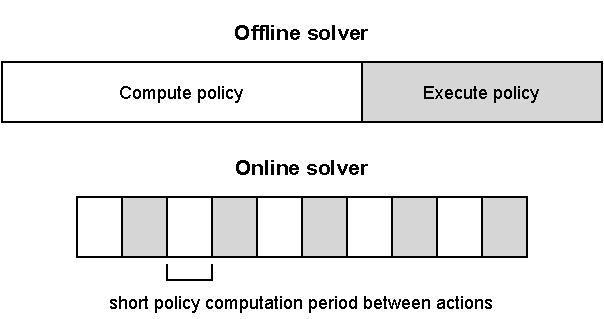
\includegraphics[width=0.6\textwidth]{figures/online-offline.pdf}
    \caption{Comparison of offline and online solving procedure}
    \label{fig:online-offline}
\end{figure}

\noindent
There are two general approaches to solve POMDP: offline and online (see figure \ref{fig:online-offline}). Offline solvers compute the optimal policy prior to execution for all possible future scenarios. Their advantage is that once the policy is determined, policy execution is fast as there is only a very minimal, negligible time overhead. However, offline planning is hard to scale to complex problems as the number of possible future scenarios grows exponentially with the size of the time horizon (curse of history). Furthermore, while the performance for small to medium-sized POMDPs can be good, computing the policy may take a very long time. Furthermore, even small changes in the dynamics of the environment require a full recomputation \parencite{online_pomdp}. Online solvers interleave planning and plan execution. At every time step, only the current belief is considered for the computation of the next optimal action by searching ahead until a certain depth is reached. On the one hand, the scalability is greatly increased. On the other hand, sufficiently more online computation than for offline planning is required. The amount of available online planning time at each time step limits the performance. 

\subsection{Overview of aproximate POMDP solvers}
\label{sec:solvers}

As discussed in section \ref{sec:curses}, finding an exact optimal policy is only feasible for small discrete POMDPs. Larger POMDPs are usually solved approximately. A wide range of offline and online approximate solvers is available. An extensive survey of possible approaches is out of scope for this thesis. A good overview over different methods is given in the book "Algorithms for Decision Making" \parencite{decision_making_book}. We focus on introducing a selection of especially noteworthy approaches at solving POMDP in this section.

For discrete POMDP, the most effective offline approximate solvers apply a form of \gls{pbvi}, where only a representative subset of the belief space is considered to approximate the value function \parencite{pomdp-point-based-value}. State of the art methods include Perseus \parencite{pomdp_perseus}, and \gls{hsvi} \parencite{solver_hsvi}. Perseus chooses belief states by randomly sampling trajectories from an initial belief \parencite{pomdp_perseus}. It is sufficiently more compute efficient than PBVI but can suffer from a slow convergence behavior \parencite{pbvi-survey}. HSVI improves on Perseus potential slow convergence in large domains by constructing a belief search tree, maintaining the order of visited beliefs to be backtrack value updates bottom-up \parencite{solver_hsvi}. Even the most advanced offline solvers reach their limit when dealing with POMDPs with large state spaces. As the state space for the shared control lane-keeping task is large, offline solvers are not considered further in this thesis. 

When it comes to online solvers, the paradigm of searching for a good policy locally for the current belief state makes them sufficiently more efficient. The general approach is to construct a search tree with the current belief as root, evaluating all possible further actions and observations. This tree can be used to efficiently generate a good approximately optimal action to perform at the current belief. The methods mainly differ in how the tree is constructed. After an action has been performed in the real environment, the agent receives a reward and observation. On this basis, it updates its belief, and the process repeats from the new belief. 

Constructing the search tree using Monte Carlo sampling has recently led to promising results for online solving of large POMDPs \parencite{pomcp}. Including all possibilities in the search tree is not feasible for deep time horizons because of the curse of history and the curse of dimensionality (see section \ref{sec:curses}). \gls{mcts} methods address this issue by using a generative model to sample state transitions and observations (see section \ref{sec:gen_model_intro}). By doing so, only a subset of histories is considered. The curse of dimensionality can be overcome in a similar fashion. Instead of evaluating all belief states, the start states for the search tree are sampled from the belief space. The number of belief states to consider can thereby be drastically reduced. 

\subsection{Online POMDP solving using Monte Carlo tree search}

The approach of using Monte Carlo sampling for both the choice of evaluated histories and estimating the belief was first applied in the \acrfull{pomcp} algorithm by \cite{pomcp}. The exploration is controlled using the \gls{ucb1} \parencite{ucb1} algorithm for action selection. The belief search tree is constructed by sampling possible action-observation trajectories. The key idea is to approximate the belief space using the same set of states sampled for the search tree construction. POMCP's belief representation eliminates the need for expensive belief update calculations. POMCP has successfully been applied to solve large POMDPs. Thus, the POMCP algorithm was selected as the solver for our problem. In section \ref{sec:pomcp}, we explain how we employed POMCP to solve the shared control lane-keeping task. 

The \gls{despot} algorithm by \cite{despot} is a similar approach that can be seen as an evolution of POMCP. DESPOT is efficient as only a fixed number of sampled scenarios are considered. A scenario is a determinized trajectory in the belief tree that is defined in advance. At every depth of the belief tree, all actions but only a subset of resulting observations are considered. Thereby, the observation space is simplified. DESPOT's main advantage over POMCP is the ability to overcome POMCP's relatively poor worst-case behavior \parencite{pomcp-worst-case} caused by the UCB1 algorithm's tendency to overfit. DESPOT circumvents this by using regularization in the value function. First, a suboptimal policy is searched using heuristic search \parencite{solver_hsvi} and then it is incrementally improved upon. Branch-and-bound pruning is performed by pruning action nodes from the tree if their expected value is lower than the lower bound of another action. There are further extensions of DESPOT: HyPDESPOT is a parallelized version of DESPOT with significant performance enhancements \parencite{hyp-despot}. DESPOT-$\alpha$ further improves DESPOT's capability to handle very large observation and state spaces \parencite{despot-a}. And DESPOT-IS applies importance sampling to account for very rare events that are hard to sample \parencite{despot-is}. Unfortunately, DESPOT and its derivatives require the observation probability $Z$ to be explicitly known. This is not feasible for the shared control lane-keeping task considered in this thesis.

\subsection{Solving continuous POMDP}

The scenario of lane-keeping with a human in the loop that we examine is naturally continuous; steering actions, car state, and sensory information about the car's position are all composed of continuous values (see section \ref{sec:lane_keeping_loop}). Hence, a solver that can handle continuous POMDP is required.

The aforementioned algorithms POMCP and DESPOT can natively handle continuous state spaces \parencite{pomcp_continuous}. It is unlikely that two identical continuous states are inserted into the collection of states representing the agent's belief. Therefore, the individual relative frequency of a state in the belief, representing its probability in the discrete case, is rendered meaningless. Nevertheless, if the agent samples multiple similar situations, the corresponding states are also similar. For the continuous case, the assumed probability of being in a certain state is given by the number of belief states close to it.

However, POMCP and DESPOT cannot be applied directly with PODMPs that have continuous action and observation spaces. Discretization is required \parencite{pomcp_continuous}. Action and observation discretization is performed in this thesis to be able to use POMCP. The details are discussed in section \ref{sec:discretization}.

Various solvers have been developed that are suitable to solve POMDP with continuous action and observation spaces without relying on discretization. To the best of our knowledge, they all require the observation probabilities $Z$ to be known explicitly and are therefore not applicable to the problem addressed in this thesis. Yet, such approaches may be advantageous in future work if the problem of unknown observation probabilities can be circumvented. Two notable solvers are POMCPOW \parencite{online_pomdp_cont}, and LABECOP \parencite{online-cont-pomdp-2}. POMCPOW is an extension of POMCP using progressive widening. It uses weighted belief updates and limits the number of observations considered during planning. LABECOP is based on MCTS as well but avoids limiting the number of considered observations.